\documentclass[12pt, a4paper]{report}

% - Encoding & Language -
\usepackage[utf8]{inputenc}
\usepackage[T5]{fontenc}
\usepackage[vietnamese]{babel}

% - Page Layout -
\usepackage[top=3cm, bottom=3cm, left=3.5cm, right=2.5cm, headheight=14pt]{geometry}
\usepackage{setspace}
\onehalfspacing

% - Math -
\usepackage{amsmath, amssymb, amsthm}
\usepackage{mathtools}

% - Graphics & Figures -
\usepackage{graphicx}
\usepackage{float}
\usepackage{subcaption}
\usepackage[table,xcdraw]{xcolor}
\usepackage{tikz}
\usetikzlibrary{shapes.geometric, arrows.meta, positioning, fit, backgrounds}

% - Tables -
\usepackage{booktabs}
\usepackage{multirow}
\usepackage{array}
\usepackage{longtable}
\usepackage{tabularx}

% - Code -
\usepackage{listings}
\usepackage{algorithm}
\usepackage{algpseudocode}

% - References & Links -
\usepackage{hyperref}
\hypersetup{
    colorlinks=true,
    linkcolor=black,
    citecolor=blue,
    urlcolor=blue
}
\usepackage[numbers, sort&compress]{natbib}

% - Header/Footer -
\usepackage{fancyhdr}
\pagestyle{fancy}
\fancyhf{}
\fancyhead[L]{\small\textit{Hệ hỗ trợ quyết định đặt hàng}}
\fancyhead[R]{\small\thepage}
\renewcommand{\headrulewidth}{0.4pt}
\fancypagestyle{plain}{%
  \fancyhf{}
  \fancyhead[R]{\small\thepage}
  \renewcommand{\headrulewidth}{0pt}
}

% - Misc -
\usepackage{enumitem}
\usepackage{caption}
\usepackage{microtype}
\usepackage{lmodern}
\usepackage{csquotes}

% - Chapter Title Style -
\usepackage{titlesec}
\titleformat{\chapter}[block]
  {\normalfont\Large\bfseries\raggedright}
  {CHƯƠNG \thechapter.}{0.5em}{\MakeUppercase}
\titlespacing*{\chapter}{0pt}{-10pt}{20pt}

% - Custom commands -
\newcommand{\Q}[1]{\ensuremath{Q_{#1}}}
\newcommand{\CR}{\ensuremath{\mathrm{CR}}}
\newcommand{\Cu}{\ensuremath{C_u}}
\newcommand{\Co}{\ensuremath{C_o}}

\definecolor{lightgray}{rgb}{0.95,0.95,0.95}
\lstset{
  backgroundcolor=\color{lightgray},
  basicstyle=\small\ttfamily,
  breaklines=true,
  frame=single,
  numbers=left,
  numberstyle=\tiny,
  language=Python,
  showstringspaces=false
}

%=============================================================
\begin{document}

% ==================== BÌA ====================
\begin{titlepage}
\begin{center}

{\large \textbf{ĐẠI HỌC BÁCH KHOA HÀ NỘI}\\[2pt]
\textbf{KHOA TOÁN TIN}}

\vspace{1.5cm}

\rule{\linewidth}{0.5mm}\\[0.4cm]
{\LARGE \bfseries HỆ HỖ TRỢ QUYẾT ĐỊNH ĐẶT HÀNG}\\[0.4cm]
{\large \bfseries DỰA TRÊN DỰ BÁO CHUỖI THỜI GIAN ĐA PHÂN VỊ\\
TỐI ƯU HÓA TỒN KHO TRONG ĐIỀU KIỆN KHÔNG CHẮC CHẮN}
\rule{\linewidth}{0.5mm}

\vspace{0.8cm}
{\large \textbf{Môn học:} Hệ hỗ trợ quyết định}\\[0.4cm]
{\large \textbf{Học kỳ:} 20252 - Năm học 2024-2025}

\vfill

\begin{flushleft}
{\large
\textbf{Thông tin sinh viên:}\\[6pt]
\begin{tabular}{ll}
Họ và tên: & Nguyễn Trường Giang, Đinh Hải Phong \\
MSSV:      & \textit{20227044} \\
Lớp:       & \textit{169317} \\
Email:     & giang.nt04@outlook.com.vn \\
\end{tabular}
}
\end{flushleft}

\vspace{0.5cm}
{\large \textbf{Giảng viên hướng dẫn:} \textit{Trần Ngọc Thăng, Lê Hải Hà}}

\vspace{0.8cm}
{\large Hà Nội, tháng 6 năm 2025}
\end{center}
\end{titlepage}

% ==================== LỜI CAM ĐOAN ====================

% ==================== TÓM TẮT ====================
\chapter*{Tóm tắt}
\addcontentsline{toc}{chapter}{Tóm tắt}

Báo cáo này trình bày thiết kế và triển khai một \textbf{Hệ hỗ trợ quyết định đặt hàng} (Decision Support System - DSS) tích hợp hai thành phần chính: (1) mô hình dự báo nhu cầu chuỗi thời gian đa phân vị và (2) mô hình tối ưu hóa tồn kho có cơ sở kinh tế.

Về dự báo, mô hình \textbf{RevIN + N-BEATS} được tự xây dựng bằng PyTorch kết hợp chuẩn hóa theo thực thể đảo ngược (Reversible Instance Normalization - RevIN) và kiến trúc N-BEATS với đầu ra đa phân vị (P5, P10, P25, P50, P75, P90, P95). Mô hình được huấn luyện bằng hàm mất mát \textit{pinball loss} - tiêu chuẩn lý thuyết cho hồi quy phân vị - và tối ưu siêu tham số bằng thuật toán Optuna (100 thử nghiệm, TPE sampler). Dữ liệu là 120 quan sát tháng (2015-2024), chia theo chiến lược thời gian 8:1:1.

Trên tập kiểm tra (2024), mô hình đạt \textbf{MAE = 3.254, MAPE = 0,97\%}, vượt trội gần \textbf{24 lần} so với phương pháp cơ sở Naive (MAE = 79.188, MAPE = 22,76\%). Về quyết định tồn kho, kết quả phân vị được đưa vào \textbf{mô hình Newsvendor} - tỷ lệ tới hạn $\CR = \Cu/(\Cu + \Co)$ xác định trực tiếp mức phân vị tối ưu cần chuẩn bị, mang ý nghĩa kinh tế rõ ràng mà dự báo điểm không thể hiện được. Mô hình \textbf{EOQ} bổ sung khuyến nghị cỡ lô cho vận hành dài hạn.

Hệ thống được triển khai dưới dạng hai ứng dụng web Streamlit: bản kỹ thuật đầy đủ chỉ số và bản dành cho người dùng kinh doanh với ngôn ngữ đời thường.

\textbf{Từ khóa:} dự báo chuỗi thời gian, N-BEATS, RevIN, hồi quy phân vị, pinball loss, newsvendor, tối ưu tồn kho, hệ hỗ trợ quyết định.

% ==================== MỤC LỤC ====================
\tableofcontents
\listoffigures
\listoftables

% ==================== CHƯƠNG 1 ====================
\chapter{Giới thiệu}

\section{Bối cảnh và động lực}

Trong quản lý chuỗi cung ứng, câu hỏi ``\textit{Tháng này nên đặt bao nhiêu hàng?}'' tưởng chừng đơn giản nhưng hàm chứa hai rủi ro đối lập: đặt ít thì hết hàng (mất doanh thu, mất khách), đặt nhiều thì tồn kho ế (ứ đọng vốn, hao hụt). Khó khăn căn bản nằm ở chỗ nhu cầu tương lai \textit{không thể biết chắc} - dự báo tốt nhất cũng chỉ cung cấp một ước lượng kèm theo mức độ không chắc chắn.

Hầu hết các hệ thống thực tế vẫn dùng \textit{dự báo điểm} (một con số duy nhất) rồi áp dụng quy tắc kinh nghiệm để tính an toàn tồn kho. Cách tiếp cận này bỏ qua một phần thông tin quan trọng: \textit{phân phối xác suất} của nhu cầu, mà chính phân phối đó mới quyết định được mức tồn kho tối ưu về kinh tế.

Báo cáo này đề xuất một hệ thống khép kín kết hợp:
\begin{enumerate}
  \item Dự báo \textbf{đa phân vị} (quantile forecasting) bằng RevIN + N-BEATS - cung cấp \textit{cả phân phối} nhu cầu thay vì một con số.
  \item Tối ưu hóa tồn kho bằng \textbf{mô hình Newsvendor} - dùng trực tiếp phân phối đó để tìm mức chuẩn bị tối ưu theo tiêu chí kinh tế.
\end{enumerate}

\section{Mục tiêu}

\begin{enumerate}
  \item Xây dựng mô hình dự báo chuỗi thời gian đa phân vị tự triển khai (RevIN + N-BEATS, PyTorch), tối ưu siêu tham số bằng Optuna.
  \item Kết nối đầu ra dự báo với mô hình Newsvendor để đưa ra khuyến nghị đặt hàng có ý nghĩa kinh tế.
  \item Triển khai hệ thống dưới dạng ứng dụng web tương tác (Streamlit) phục vụ hai nhóm người dùng: kỹ thuật viên phân tích và quản lý kinh doanh.
\end{enumerate}

\section{Phạm vi và đóng góp}

\begin{itemize}
  \item \textbf{Dữ liệu:} chuỗi thời gian doanh số tháng thực tế, 120 quan sát (2015-2024), cùng 10 biến ngoại sinh vĩ mô.
  \item \textbf{Đóng góp kỹ thuật:} (i) đầu ra đơn điệu đa phân vị trong N-BEATS qua tham số hóa softplus-cumsum; (ii) chuẩn hóa RevIN 3D tương thích với tensor đầu ra $(\text{batch} \times \text{horizon} \times Q)$; (iii) tích hợp mô hình Newsvendor từ phân vị rời rạc qua nội suy.
  \item \textbf{Đóng góp ứng dụng:} hai giao diện web phục vụ hai đối tượng với ngôn ngữ và mức độ chi tiết khác nhau.
\end{itemize}

\section{Cấu trúc báo cáo}

Báo cáo gồm 5 chương: Chương 2 trình bày cơ sở lý thuyết; Chương 3 mô tả dữ liệu và phương pháp; Chương 4 trình bày kết quả thực nghiệm; Chương 5 kết luận và định hướng phát triển.

% ==================== CHƯƠNG 2 ====================
\chapter{Cơ sở lý thuyết}

\section{Dự báo chuỗi thời gian}

\subsection{Bài toán dự báo điểm và dự báo phân vị}

Cho chuỗi thời gian $y_1, y_2, \ldots, y_T$. Dự báo điểm tìm hàm $\hat{y}_{T+h} = f(y_1,\ldots,y_T)$ nhằm tối thiểu hóa một sai số như MAE hoặc MSE. Dự báo phân vị bậc $q \in (0,1)$ tìm $\hat{F}^{-1}(q)$ sao cho xác suất thực tế $y_{T+h} \leq \hat{F}^{-1}(q)$ xấp xỉ $q$:
\begin{equation}
  P\!\left(y_{T+h} \leq \hat{F}^{-1}(q)\right) \approx q.
\end{equation}
Dự báo đồng thời nhiều phân vị cho phép ước lượng \textit{toàn bộ phân phối} nhu cầu mà không cần giả thiết tham số (Gaussian, v.v.).

\subsection{Hàm mất mát Pinball (Quantile Loss)}

Để huấn luyện mô hình dự báo phân vị, hàm mất mát pinball (còn gọi là quantile loss) được định nghĩa \cite{koenker1978regression}:
\begin{equation}
  \mathcal{L}_q(\hat{y}, y) = \max\!\bigl[q(y - \hat{y}),\; (q-1)(y - \hat{y})\bigr],
\end{equation}
hay tương đương:
\begin{equation}
  \mathcal{L}_q(\hat{y}, y) =
  \begin{cases}
    q\,(y - \hat{y})   & \text{nếu } y \geq \hat{y}, \\
    (q-1)(y - \hat{y}) & \text{nếu } y < \hat{y}.
  \end{cases}
\end{equation}
Với tập phân vị $\mathcal{Q} = \{q_1, \ldots, q_K\}$, tổng pinball loss trung bình:
\begin{equation}
  \mathcal{L} = \frac{1}{NK} \sum_{i=1}^{N} \sum_{k=1}^{K} \mathcal{L}_{q_k}(\hat{y}_{i,q_k},\, y_i).
\end{equation}
Hàm này phạt bất đối xứng theo $q$: phân vị cao ($q$ lớn) phạt nặng khi dự báo \textit{thấp hơn} thực tế, và ngược lại.

\section{Reversible Instance Normalization (RevIN)}

\subsection{Vấn đề phân phối trôi dạt (Distribution Shift)}

Chuỗi thời gian thực tế thường có phân phối thay đổi theo thời gian - xu hướng, mùa vụ, hoặc thay đổi cấu trúc (structural break). Mô hình học trên dữ liệu cũ ($\mu_{\text{train}}, \sigma_{\text{train}}$) sẽ gặp khó khăn khi dự báo giai đoạn mới có $\mu_{\text{test}} \neq \mu_{\text{train}}$.

\subsection{Cơ chế RevIN}

RevIN \cite{kim2022reversible} chuẩn hóa \textit{từng cửa sổ đầu vào} (instance) theo mean/std của chính nó, thay vì dùng thống kê toàn cục:

\textbf{Bước chuẩn hóa (normalize):}
\begin{equation}
  \hat{x}_t = \frac{x_t - \hat{\mu}}{\hat{\sigma} + \varepsilon}, \quad
  \hat{\mu} = \frac{1}{L}\sum_{t=1}^{L} x_t, \quad
  \hat{\sigma} = \sqrt{\frac{1}{L}\sum_{t=1}^{L}(x_t - \hat{\mu})^2 + \varepsilon}.
\end{equation}

Với tham số affine học được $\gamma, \beta$ (tùy chọn):
\begin{equation}
  \tilde{x}_t = \gamma \cdot \hat{x}_t + \beta.
\end{equation}

\textbf{Bước đảo ngược (denormalize):} Sau khi mạng tạo dự báo $\hat{y}$ ở không gian chuẩn hóa, chuyển về thang đo gốc:
\begin{equation}
  y = \hat{y} \cdot \hat{\sigma} + \hat{\mu}.
\end{equation}

Với đầu ra đa phân vị $(\text{batch} \times H \times Q)$, phép denormalize mở rộng:
\begin{equation}
  \mathbf{Y}_{b,h,q} = \hat{\mathbf{Y}}_{b,h,q} \cdot \hat{\sigma}_b + \hat{\mu}_b,
\end{equation}
trong đó $\hat{\sigma}_b, \hat{\mu}_b$ được broadcast theo chiều batch.

\section{N-BEATS}

\subsection{Kiến trúc tổng quan}

N-BEATS \cite{oreshkin2019n} là mạng nơ-ron thuần (fully-connected) không hồi quy theo chuỗi (recurrence-free), gồm nhiều \textit{stack}, mỗi stack gồm nhiều \textit{block}. Kiến trúc sử dụng cơ chế \textbf{doubly-residual stacking}: mỗi block nhận tín hiệu dư từ block trước, trừ đi backcast và cộng dồn forecast.

\subsection{Block N-BEATS}

Mỗi block là một MLP gồm $n_{\text{layers}}$ lớp ẩn với ReLU:
\begin{align}
  \mathbf{h}_1 &= \text{ReLU}(\mathbf{W}_1 \mathbf{x} + \mathbf{b}_1), \\
  \mathbf{h}_l &= \text{ReLU}(\mathbf{W}_l \mathbf{h}_{l-1} + \mathbf{b}_l), \quad l=2,\ldots,n_{\text{layers}}.
\end{align}

Block xuất ra hai đầu:
\begin{align}
  \hat{\mathbf{x}}_{\text{back}} &= \mathbf{W}_{\text{back}} \mathbf{h}, \quad \in \mathbb{R}^L \quad \text{(backcast)}, \\
  \hat{\mathbf{y}}_{\text{fore}} &= \mathbf{W}_{\text{fore}} \mathbf{h}, \quad \in \mathbb{R}^{H \times K} \quad \text{(forecast đa phân vị)}.
\end{align}

\subsection{Ràng buộc đơn điệu phân vị (Monotone Quantile Head)}

Để đảm bảo $\hat{F}^{-1}(q_1) \leq \hat{F}^{-1}(q_2)$ với mọi $q_1 < q_2$ (không bị \textit{quantile crossing}), đầu ra được tham số hóa qua cumsum-softplus \cite{chung2021beyond}:
\begin{align}
  \hat{y}_{h,0} &= \mathbf{W}_0 \mathbf{h} \quad \text{(phân vị thấp nhất, P5)}, \\
  \hat{y}_{h,k} &= \hat{y}_{h,0} + \sum_{j=1}^{k} \text{softplus}(\mathbf{W}_j \mathbf{h}), \quad k=1,\ldots,K-1.
\end{align}
Vì $\text{softplus}(z) > 0$ với mọi $z$, cumsum luôn tăng đơn điệu, đảm bảo $P5 \leq P10 \leq \cdots \leq P95$.

\subsection{Doubly-Residual Stacking}

Với $n_{\text{blocks}}$ block trong một stack:
\begin{align}
  \mathbf{x}^{(1)} &= \mathbf{x}_{\text{in}}, \\
  \mathbf{x}^{(l+1)} &= \mathbf{x}^{(l)} - \hat{\mathbf{x}}^{(l)}_{\text{back}}, \\
  \hat{\mathbf{Y}}_{\text{stack}} &= \sum_{l=1}^{n_{\text{blocks}}} \hat{\mathbf{y}}^{(l)}_{\text{fore}}.
\end{align}

Qua $n_{\text{stacks}}$ stack tương tự:
\begin{equation}
  \hat{\mathbf{Y}}_{\text{final}} = \sum_{s=1}^{n_{\text{stacks}}} \hat{\mathbf{Y}}_s.
\end{equation}

\section{Tối ưu siêu tham số bằng Optuna}

Optuna \cite{akiba2019optuna} sử dụng thuật toán \textit{Tree-structured Parzen Estimator} (TPE): xây dựng mô hình xác suất $p(x|y<y^*)$ (phân phối siêu tham số dẫn đến kết quả tốt) và $p(x|y \geq y^*)$, rồi chọn điểm tối đa tỷ số $p(x|y<y^*) / p(x|y \geq y^*)$ để thử nghiệm tiếp theo.

\textit{MedianPruner} dừng sớm trial nếu giá trị mục tiêu tại bước hiện tại tệ hơn trung vị của các trial hoàn thành trước - tiết kiệm tài nguyên tính toán.

\section{Mô hình Newsvendor}

\subsection{Bài toán}

Bài toán Newsvendor (người bán báo) \cite{arrow1951optimal} xét việc đặt hàng một kỳ với nhu cầu ngẫu nhiên $D \sim F$. Nếu đặt $Q$ đơn vị:
\begin{itemize}
  \item Nếu $D > Q$: thiếu $(D - Q)$ đơn vị, mỗi đơn vị thiệt hại $\Cu$ (lợi nhuận mất).
  \item Nếu $D < Q$: thừa $(Q - D)$ đơn vị, mỗi đơn vị thiệt hại $\Co$ (chi phí tồn kho).
\end{itemize}

\subsection{Mức tồn kho tối ưu}

Tổng chi phí kỳ vọng:
\begin{equation}
  TC(Q) = \Cu \cdot \mathbb{E}[\max(D-Q, 0)] + \Co \cdot \mathbb{E}[\max(Q-D, 0)].
\end{equation}

Tối thiểu hóa $TC(Q)$ cho kết quả \cite{porteus2002foundations}:
\begin{equation}
  \boxed{Q^* = F^{-1}(\CR), \qquad \CR = \frac{\Cu}{\Cu + \Co}.}
\end{equation}

$\CR$ được gọi là \textbf{tỷ lệ tới hạn} (critical ratio) - đồng thời là mức phân vị tối ưu của phân phối nhu cầu. Ý nghĩa kinh tế rõ ràng:
\begin{itemize}
  \item Sản phẩm lãi cao ($\Cu \gg \Co$) $\Rightarrow$ $\CR \to 1$ $\Rightarrow$ chuẩn bị ở phân vị cao (P90, P95), chấp nhận ít khi hết hàng.
  \item Sản phẩm dễ ế/chi phí tồn cao ($\Co \gg \Cu$) $\Rightarrow$ $\CR \to 0$ $\Rightarrow$ chuẩn bị ở phân vị thấp, chấp nhận đôi khi cháy hàng.
\end{itemize}

\subsection{Kết hợp với dự báo phân vị}

Khi $F$ được ước lượng từ mô hình dự báo phân vị rời rạc $\{(q_k, \hat{F}^{-1}(q_k))\}$, $Q^*$ được tính bằng nội suy tuyến tính:
\begin{equation}
  Q^* = \hat{F}^{-1}(\CR) = \text{interp}\!\left(\CR;\; [q_1,\ldots,q_K],\; [\hat{y}_{q_1},\ldots,\hat{y}_{q_K}]\right).
\end{equation}

\section{Mô hình EOQ}

Mô hình Economic Order Quantity \cite{harris1913many} tối ưu cỡ lô đặt hàng cho vận hành liên tục:
\begin{equation}
  Q^*_{\text{EOQ}} = \sqrt{\frac{2DS}{H}},
\end{equation}
trong đó $D$ = nhu cầu năm, $S$ = chi phí một lần đặt, $H$ = chi phí lưu kho/đơn vị/năm.

Tồn kho an toàn: $\text{SS} = z \cdot \sigma \cdot \sqrt{L}$, điểm đặt hàng lại: $\text{ROP} = \bar{d} \cdot L + \text{SS}$.

% ==================== CHƯƠNG 3 ====================
\chapter{Dữ liệu và Phương pháp}

\section{Mô tả dữ liệu}

\subsection{Tổng quan}

Tập dữ liệu gồm \textbf{120 quan sát tháng} (từ tháng 1/2015 đến tháng 12/2024), bao gồm:
\begin{itemize}
  \item \textbf{Biến mục tiêu:} \texttt{Quantity} - lượng tiêu thụ (hoặc nhu cầu) hàng tháng.
  \item \textbf{10 biến ngoại sinh vĩ mô:} CompetitorQuantity, PromotionAmount, Construction, CPI, Exports, Imports, IPI, RegisteredFDI, DisbursedFDI, RetailSales.
\end{itemize}

Thống kê mô tả chi tiết của chuỗi \texttt{Quantity} được trình bày tại Bảng~\ref{tab:desc} (mục~\ref{sec:eda_overview}).

\subsection{Đặc điểm chuỗi}

Chuỗi \texttt{Quantity} thể hiện: (i) dao động mạnh theo tháng (không có mùa vụ rõ rệt); (ii) phân phối trôi dạt nhẹ giữa giai đoạn 2015-2018 và 2019-2024; (iii) tác động đột biến của COVID-19 năm 2020-2021. Đây là lý do chính để áp dụng RevIN thay vì chuẩn hóa toàn cục.

Đặc biệt, biến \texttt{PromotionAmount} tăng gần 100 lần trong 10 năm, minh chứng rõ cho tình trạng distribution shift nghiêm trọng nếu không xử lý.

\subsection{Chiến lược chia dữ liệu}

Dữ liệu được chia theo thứ tự thời gian (không xáo trộn) theo tỷ lệ 8:1:1:

\begin{table}[H]
\centering
\caption{Chiến lược chia dữ liệu 8:1:1 theo thời gian}
\label{tab:split}
\begin{tabular}{|l|l|r|r|}
\hline
Tập & Khoảng thời gian & Số quan sát & Tỷ lệ \\
\hline
Train      & 2015-01 $\to$ 2022-12 & 96  & 80\% \\
Validation & 2023-01 $\to$ 2023-12 & 12  & 10\% \\
Test       & 2024-01 $\to$ 2024-12 & 12  & 10\% \\
\hline
\end{tabular}
\end{table}

Tập validation dùng để tối ưu siêu tham số (Optuna) và chọn early stopping. Tập test được đánh giá \textit{một lần duy nhất} sau khi chọn mô hình cuối cùng.

% --------------
\section{Phân tích khám phá dữ liệu (EDA)}
% --------------

\subsection{Tổng quan chuỗi thời gian}\label{sec:eda_overview}

Hình~\ref{fig:series_split} hiển thị chuỗi \texttt{Quantity} trong suốt 10 năm (2015-2024) cùng với ranh giới phân chia 3 tập dữ liệu. Chuỗi dao động mạnh quanh mức trung bình $\bar{y} = 349{,}023$ đơn vị, với hệ số biến thiên $\text{CV} = 21{,}3\%$ - cho thấy nhu cầu không ổn định theo thời gian.

\begin{figure}[H]
  \centering
  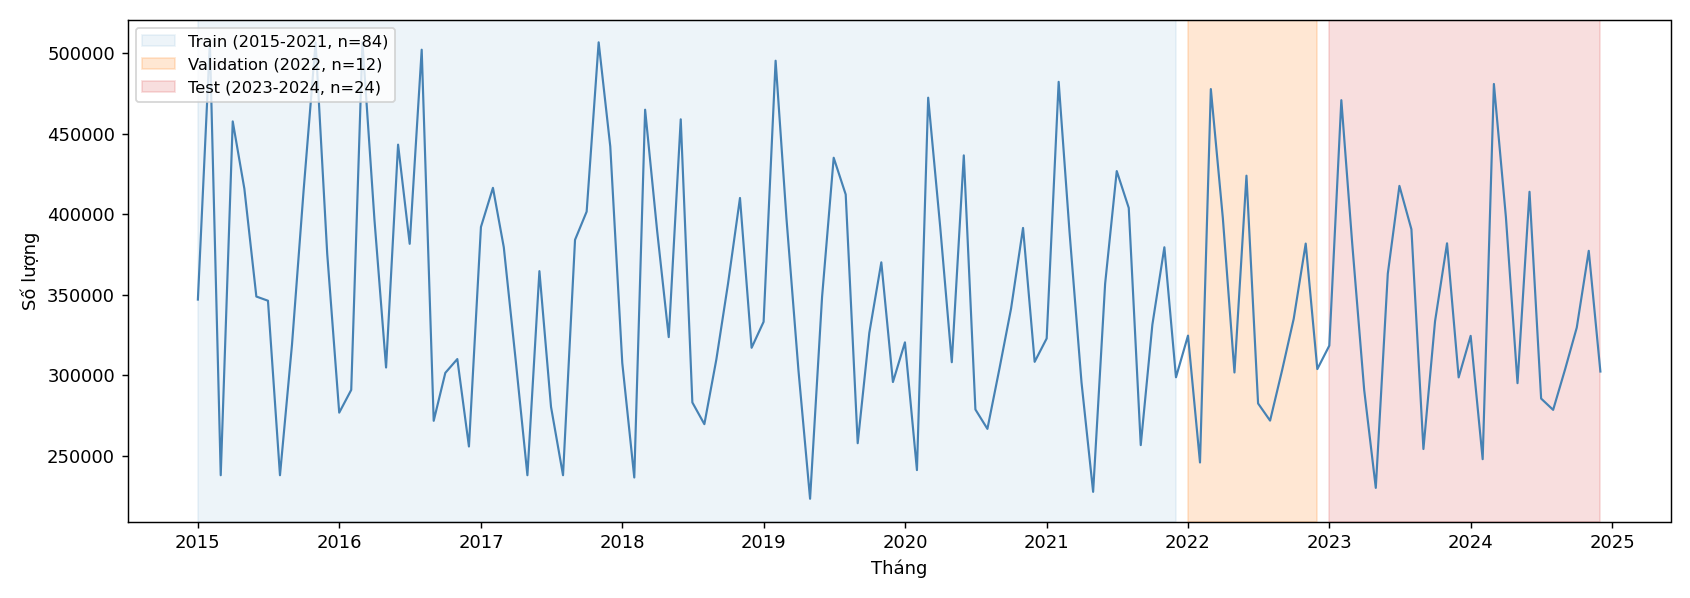
\includegraphics[width=\linewidth]{figures/fig1_series_split.png}
  \caption{Chuỗi thời gian Quantity và phân chia tập train/validation/test theo thời gian.}
  \label{fig:series_split}
\end{figure}

\begin{table}[H]
\centering
\caption{Thống kê mô tả chuỗi \texttt{Quantity} (n = 120 tháng)}
\label{tab:desc}
\begin{tabular}{|l|r|r|r|r|r|r|r|r|}
\hline
 & Min & Q1 & Trung vị & Trung bình & Q3 & Max & Std & CV \\
\hline
Quantity & 223.131 & 295.639 & 333.287 & 349.023 & 397.814 & 506.905 & 74.362 & 21,3\% \\
\hline
\end{tabular}
\end{table}

\subsection{Phân tích phân phối}

Hình~\ref{fig:distribution} cho thấy phân phối \texttt{Quantity} có độ lệch phải nhẹ ($\text{Skewness} = 0{,}377$) và đuôi mỏng hơn chuẩn ($\text{Kurtosis} = -0{,}716$). Đồ thị Q-Q xác nhận phân phối xấp xỉ chuẩn với hệ số tương quan $r = 0{,}985$, nhưng có hai đuôi lệch nhẹ so với đường lý tưởng.

\begin{figure}[H]
  \centering
  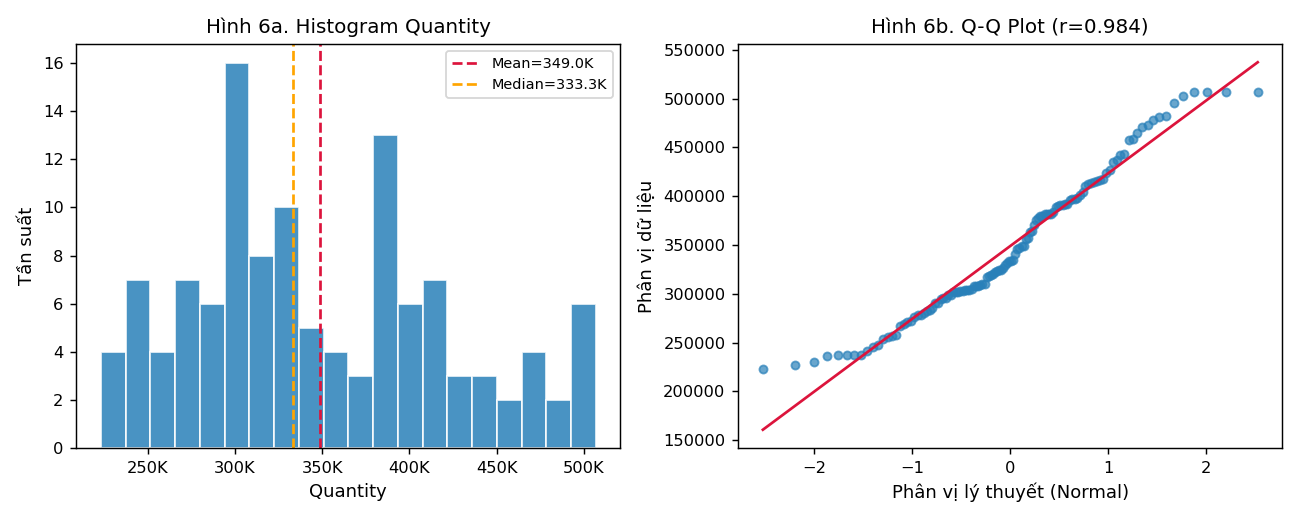
\includegraphics[width=\linewidth]{figures/fig6_distribution.png}
  \caption{Histogram và Q-Q plot của chuỗi Quantity. Skewness = 0,377; Kurtosis = -0,716.}
  \label{fig:distribution}
\end{figure}

\subsection{Kiểm định tính dừng}

Hai kiểm định được thực hiện trên chuỗi gốc:

\begin{itemize}
  \item \textbf{ADF (Augmented Dickey-Fuller):} $\text{stat} = -3{,}446$, $p = 0{,}0095 < 0{,}05$ \\
    $\Rightarrow$ \textit{bác bỏ} giả thuyết không (có nghiệm đơn vị) - chuỗi \textbf{có tính dừng}.
  \item \textbf{KPSS:} $\text{stat} = 0{,}481$, $p = 0{,}046 < 0{,}05$ \\
    $\Rightarrow$ \textit{bác bỏ} giả thuyết không (chuỗi dừng) - cho thấy tồn tại \textbf{xu hướng cục bộ}.
\end{itemize}

Hai kết quả mâu thuẫn nhau là hiện tượng phổ biến với chuỗi có xu hướng yếu: ADF có đủ bằng chứng bác bỏ nghiệm đơn vị toàn cục, nhưng KPSS vẫn phát hiện cấu trúc thay đổi cục bộ. Điều này củng cố quyết định dùng RevIN (chuẩn hóa theo từng cửa sổ) thay vì differencing toàn cục.

\subsection{Phân rã STL}

Phân rã STL (Seasonal-Trend decomposition using LOESS) tách chuỗi thành ba thành phần (Hình~\ref{fig:stl}):

\begin{itemize}
  \item \textbf{Xu hướng:} tăng nhẹ từ 2015 đến 2018, sau đó biến động mạnh trong giai đoạn 2019-2021 (ảnh hưởng COVID-19), phục hồi dần từ 2022.
  \item \textbf{Mùa vụ:} biên độ dao động mùa vụ nhỏ (khoảng $\pm 20{,}000$ đơn vị), không có chu kỳ cố định rõ rệt - đây là lý do N-BEATS generic (không có module xu hướng/mùa vụ cứng) phù hợp hơn các mô hình truyền thống.
  \item \textbf{Phần dư:} phần dư lớn quanh năm 2019-2021, phản ánh các cú sốc nhu cầu không thể giải thích bằng xu hướng hay mùa vụ.
\end{itemize}

\begin{figure}[H]
  \centering
  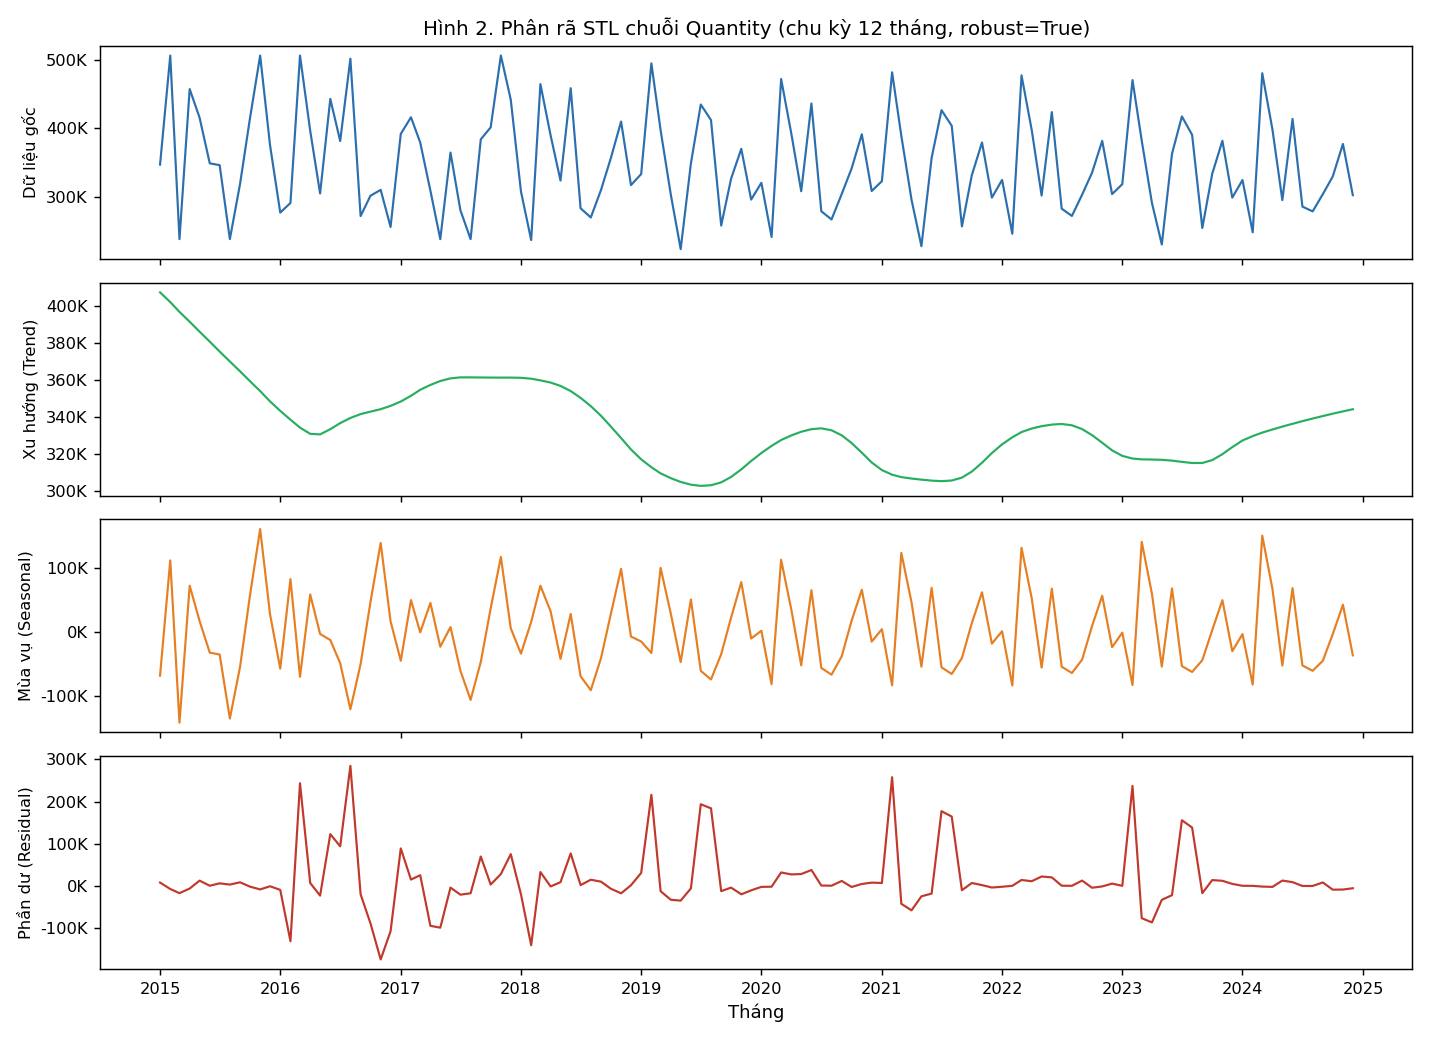
\includegraphics[width=\linewidth]{figures/fig2_stl.png}
  \caption{Phân rã STL chuỗi Quantity. Mùa vụ biên độ nhỏ; xu hướng biến động sau 2019.}
  \label{fig:stl}
\end{figure}

\subsection{Phân tích tự tương quan (ACF / PACF)}

Hình~\ref{fig:acf_pacf} cho thấy:

\begin{itemize}
  \item \textbf{ACF:} hệ số tự tương quan ở lag 1 ($\rho_1 \approx 0{,}15$) không có ý nghĩa thống kê mạnh; không có mẫu hình suy giảm chậm - phù hợp với chuỗi dừng.
  \item \textbf{PACF:} không có lag nào vượt ngưỡng ý nghĩa rõ ràng; gợi ý rằng các mô hình AR bậc thấp ($p \leq 2$) có thể không đủ để nắm bắt cấu trúc.
  \item Không có spike rõ tại lag 12/24, xác nhận mùa vụ yếu như phân rã STL đã chỉ ra.
\end{itemize}

Kết luận: chuỗi không có cấu trúc AR/MA đơn giản, cần mô hình linh hoạt như N-BEATS để học các mẫu phi tuyến.

\begin{figure}[H]
  \centering
  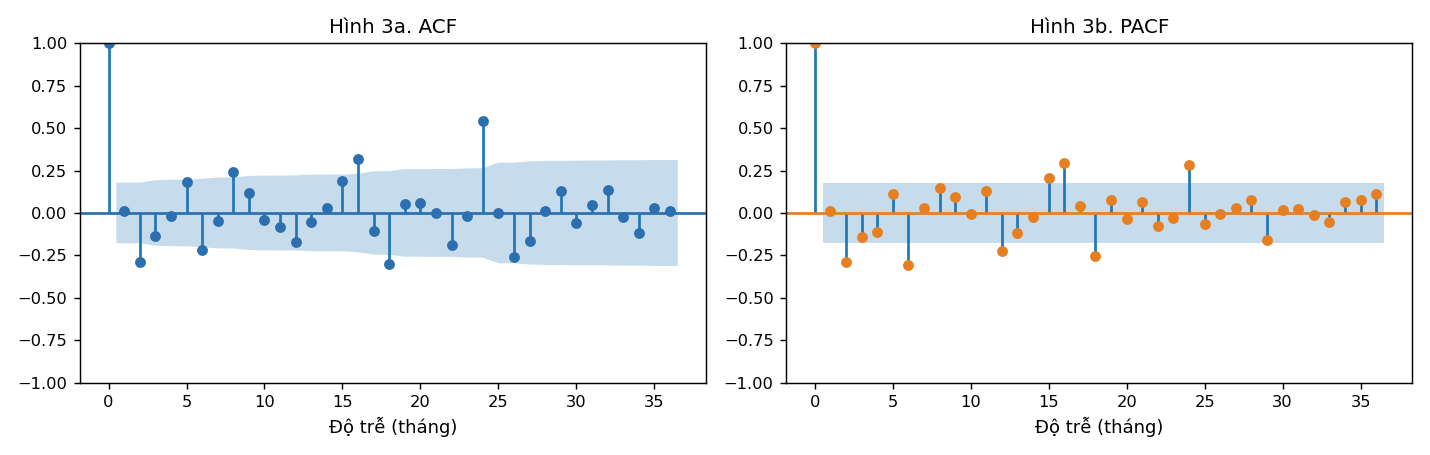
\includegraphics[width=\linewidth]{figures/fig3_acf_pacf.png}
  \caption{ACF và PACF của chuỗi Quantity. Không có cấu trúc AR/MA rõ ràng.}
  \label{fig:acf_pacf}
\end{figure}

\subsection{Phân tích mùa vụ theo tháng}

Hình~\ref{fig:boxplot} so sánh phân phối nhu cầu theo từng tháng trong năm (gộp tất cả các năm). Nhận xét:

\begin{itemize}
  \item Tháng 2 có xu hướng thấp nhất (tháng ngắn, Tết Nguyên Đán).
  \item Tháng 3 có trung vị cao nhất và biến thiên lớn nhất.
  \item Hầu hết các tháng có IQR chồng lên nhau đáng kể - hiệu ứng mùa vụ không đủ mạnh để giải thích phần lớn biến động.
\end{itemize}

\begin{figure}[H]
  \centering
  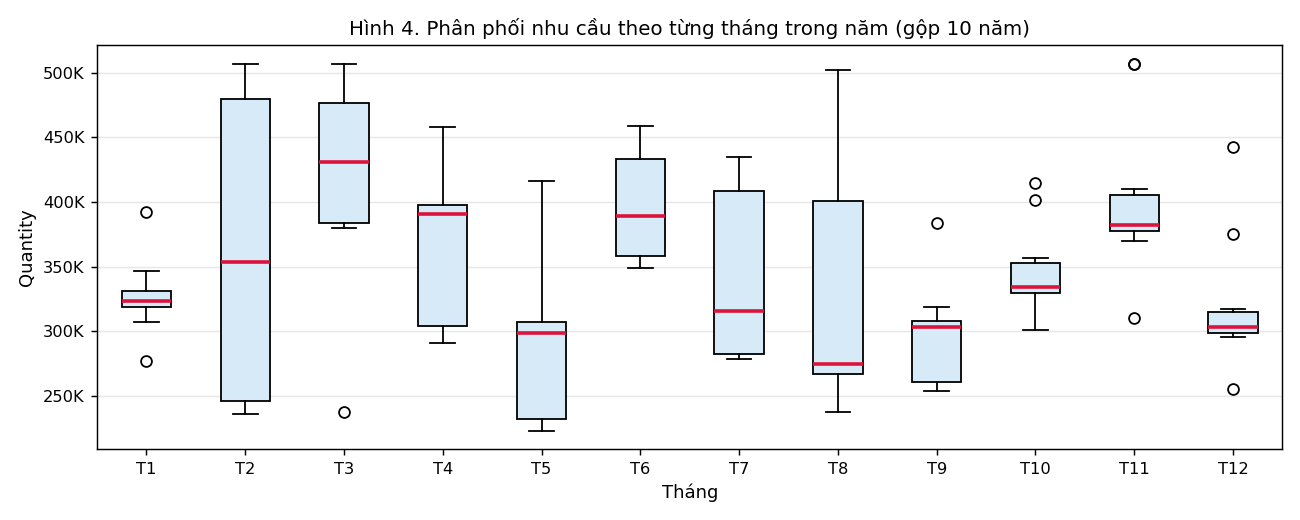
\includegraphics[width=0.95\linewidth]{figures/fig4_boxplot_month.png}
  \caption{Box plot phân phối Quantity theo từng tháng trong năm (gộp 2015-2024).}
  \label{fig:boxplot}
\end{figure}

\subsection{Tương quan với biến ngoại sinh}

Hình~\ref{fig:correlation} cho thấy hệ số tương quan Pearson giữa 10 biến ngoại sinh và \texttt{Quantity}. Nhận xét:

\begin{itemize}
  \item \textbf{IPI} (chỉ số sản xuất công nghiệp) có tương quan dương cao nhất ($r = +0{,}300$) - nhu cầu tăng khi sản xuất tăng.
  \item \textbf{Imports} ($r = +0{,}244$): nhập khẩu tăng kèm nhu cầu tăng, có thể phản ánh mối liên hệ qua chuỗi cung ứng.
  \item \textbf{PromotionAmount} ($r \approx -0{,}007$) và \textbf{CompetitorQuantity} ($r = +0{,}087$): tương quan rất thấp, bất ngờ vì đây là các biến thường được kỳ vọng có ảnh hưởng lớn.
  \item Tất cả các hệ số $|r| < 0{,}35$ - không có biến ngoại sinh nào tương quan tuyến tính mạnh với nhu cầu.
\end{itemize}

Điều này giải thích tại sao mô hình đơn biến (univariate) vẫn hoạt động tốt: thông tin từ các biến ngoại sinh không cung cấp tín hiệu tuyến tính rõ về nhu cầu. Mối quan hệ có thể tồn tại nhưng ở dạng phi tuyến hoặc có độ trễ, đòi hỏi các kiến trúc phức tạp hơn để khai thác.

\begin{figure}[H]
  \centering
  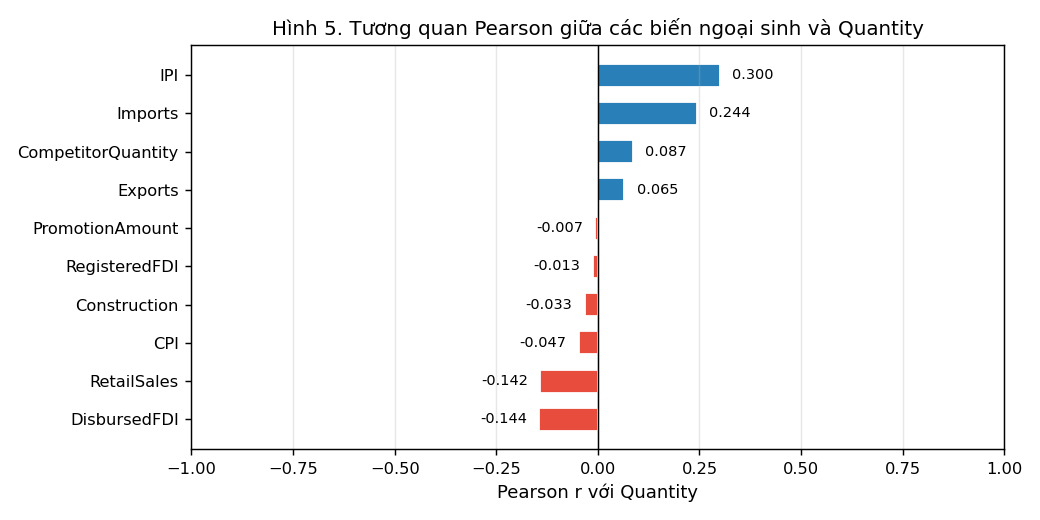
\includegraphics[width=0.9\linewidth]{figures/fig5_correlation.png}
  \caption{Hệ số tương quan Pearson giữa các biến ngoại sinh và Quantity. IPI và Imports có tương quan dương cao nhất.}
  \label{fig:correlation}
\end{figure}

\subsection{Distribution Shift}

Hình~\ref{fig:exog_trend} minh họa rõ ràng hiện tượng distribution shift qua hai biến ngoại sinh:

\begin{itemize}
  \item \textbf{PromotionAmount} tăng từ $\sim 3$ tỷ đồng/tháng (2015) lên $\sim 296$ tỷ đồng/tháng (2024) - tăng gần \textbf{90 lần} trong 10 năm. Đây là phân phối trôi dạt cực đoan.
  \item \textbf{CompetitorQuantity} tăng đơn điệu từ $\sim 1{,}1$ triệu lên $\sim 4{,}3$ triệu - tăng gần 4 lần.
\end{itemize}

Nếu dùng chuẩn hóa toàn cục (mean/std trên toàn bộ dataset), mô hình sẽ thấy giá trị PromotionAmount năm 2015 ở mức $-0{,}6\sigma$ và năm 2024 ở mức $+5\sigma$ - gây ra vấn đề nghiêm trọng khi dự báo. RevIN giải quyết đúng điểm này bằng cách chuẩn hóa từng cửa sổ riêng lẻ.

\begin{figure}[H]
  \centering
  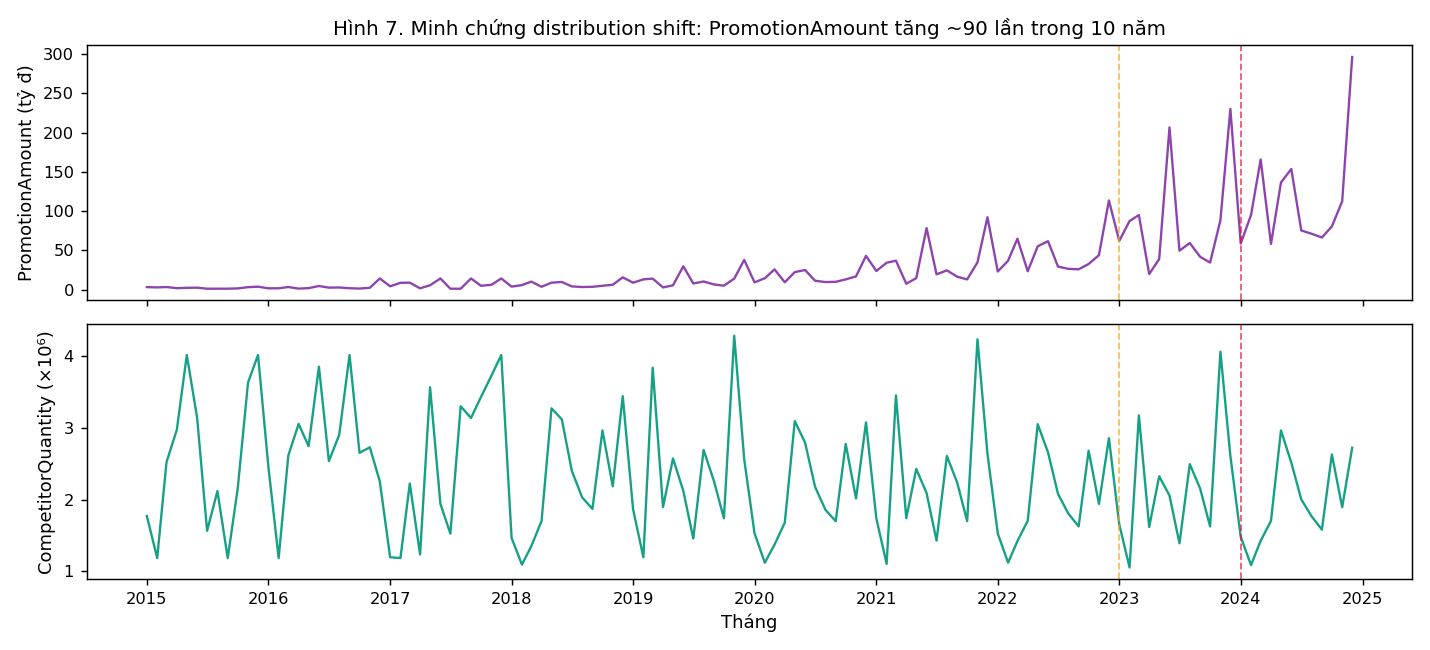
\includegraphics[width=\linewidth]{figures/fig7_exog_trend.png}
  \caption{Distribution shift rõ rệt: PromotionAmount tăng $\sim$90 lần và CompetitorQuantity tăng $\sim$4 lần trong 10 năm. Đường đứt: ranh giới train/val/test.}
  \label{fig:exog_trend}
\end{figure}

\subsection{Tóm tắt phát hiện EDA}

\begin{table}[H]
\centering
\caption{Tóm tắt phát hiện EDA và lựa chọn phương pháp}
\label{tab:eda_summary}
\renewcommand{\arraystretch}{1.4}
\begin{tabular}{|
  >{\raggedright\arraybackslash}p{0.33\linewidth}|
  >{\raggedright\arraybackslash}p{0.33\linewidth}|
  >{\raggedright\arraybackslash}p{0.21\linewidth}|
}
\hline
\rowcolor{gray!18}
\textbf{Phát hiện} & \textbf{Ý nghĩa} & \textbf{Phương pháp xử lý} \\
\hline
Chuỗi dừng yếu (ADF/KPSS mâu thuẫn)
  & Không cần differencing, nhưng có drift cục bộ
  & RevIN per-instance \\
\hline
Mùa vụ biên độ nhỏ, không ổn định
  & Mô hình mùa vụ cứng kém hiệu quả
  & N-BEATS generic \\
\hline
Không có cấu trúc AR/MA rõ ràng
  & ARIMA/ETS kém hiệu quả với chuỗi phi tuyến
  & MLP phi tuyến (N-BEATS) \\
\hline
Distribution shift nghiêm trọng (PromotionAmount $\times 90$ lần)
  & Chuẩn hóa toàn cục sẽ gây sai lệch lớn
  & RevIN per-instance \\
\hline
Tương quan tuyến tính biến ngoại sinh thấp ($|r| < 0{,}35$)
  & Biến ngoại sinh không cải thiện nhiều ở dạng tuyến tính
  & Mô hình đơn biến \\
\hline
CV $= 21{,}3\%$ - nhu cầu dao động lớn
  & Dự báo điểm đơn lẻ không đủ cho quyết định tồn kho
  & Quantile forecasting \\
\hline
\end{tabular}
\end{table}

\section{Kiến trúc hệ thống}

Hình~\ref{fig:pipeline} mô tả kiến trúc tổng thể của hệ thống.

\begin{figure}[H]
\centering
\resizebox{\linewidth}{!}{%
\begin{tikzpicture}[
  box/.style={draw, rounded corners=4pt, fill=blue!10,
              text width=2.4cm, align=center,
              minimum height=1.1cm, font=\small},
  gbox/.style={draw, rounded corners=4pt, fill=green!12,
               text width=2.4cm, align=center,
               minimum height=1.1cm, font=\small},
  obox/.style={draw, rounded corners=4pt, fill=orange!20,
               text width=2.4cm, align=center,
               minimum height=1.1cm, font=\small},
  arr/.style={->, >=Stealth, thick, shorten >=2pt, shorten <=2pt},
  node distance=0.5cm and 0.45cm
]
  % - Hang tren: pipeline du bao -
  \node[box] (data)   {Dữ liệu\\tháng (120 obs)};
  \node[box, right=of data]   (revin)  {RevIN\\Normalize};
  \node[box, right=of revin]  (nbeats) {N-BEATS\\(đa phân vị)};
  \node[box, right=of nbeats] (denorm) {RevIN\\Denormalize};
  \node[box, right=of denorm] (quant)  {Phân vị\\P5-P95};

  % - Hang duoi: ton kho + app -
  \node[gbox, below=1.4cm of quant] (nv)  {Newsvendor\\$Q^* = F^{-1}(\CR)$};
  \node[gbox, left=of nv]           (eoq) {EOQ\\$Q^*_{\text{EOQ}}$};
  \node[obox, left=of eoq]          (app) {Web App\\(Streamlit)};

  % - Mui ten -
  \draw[arr] (data)   -- (revin);
  \draw[arr] (revin)  -- (nbeats);
  \draw[arr] (nbeats) -- (denorm);
  \draw[arr] (denorm) -- (quant);
  \draw[arr] (quant)  -- (nv);
  \draw[arr] (nv)     -- (eoq);
  \draw[arr] (eoq)    -- (app);
\end{tikzpicture}%
}
\caption{Kiến trúc tổng thể của hệ hỗ trợ quyết định đặt hàng}
\label{fig:pipeline}
\end{figure}

\section{Thiết lập thực nghiệm}

\subsection{Dữ liệu huấn luyện}

Chuỗi \texttt{Quantity} được scale toàn cục bằng trung bình tập train ($s = 351{,}189$) trước khi đưa vào mô hình (để ổn định gradient). RevIN sau đó chuẩn hóa từng cửa sổ riêng lẻ ở cấp độ instance.

Cửa sổ trượt (sliding window) tạo mẫu huấn luyện: input $L$ tháng → dự báo 1 tháng tiếp theo ($H=1$).

\subsection{Không gian tìm kiếm siêu tham số}

\begin{table}[H]
\centering
\caption{Không gian tìm kiếm siêu tham số (Optuna, 100 trial)}
\label{tab:search}
\begin{tabular}{|l|l|l|}
\hline
Tham số & Khoảng & Kiểu \\
\hline
\texttt{lookback} ($L$)       & 6 - 24 tháng          & int \\
\texttt{n\_stacks}             & 1 - 3                  & int \\
\texttt{n\_blocks}/stack       & 1 - 4                  & int \\
\texttt{hidden\_size}          & 64 - 512 (bước 64)     & int \\
\texttt{n\_layers}/block       & 2 - 4                  & int \\
\texttt{learning\_rate}        & $10^{-4}$ - $10^{-2}$  & float (log) \\
\texttt{batch\_size}           & \{8, 16, 32\}           & categorical \\
\texttt{dropout}               & 0 - 0.3                & float \\
\texttt{revin\_affine}         & \{True, False\}         & categorical \\
\hline
\end{tabular}
\end{table}

\subsection{Quy trình huấn luyện cuối}

\begin{enumerate}
  \item Optuna tìm tham số tốt nhất (minimize pinball loss trên validation).
  \item Huấn luyện lại với tham số tốt nhất để xác định số epoch tối ưu (early stopping trên val).
  \item Huấn luyện lại lần cuối trên train+val, số epoch cố định từ bước 2.
  \item Đánh giá \textit{một lần duy nhất} trên test.
\end{enumerate}

\subsection{Dự báo đệ quy 12 tháng}

Để tạo dự báo phân vị cho 12 tháng tới (2025), mô hình sử dụng phương pháp dự báo đệ quy: tại mỗi bước, trung vị P50 của dự báo được đưa lại làm đầu vào cho bước tiếp theo:

\begin{equation}
  \hat{\mathbf{q}}_{T+h} = \text{Model}\!\left([\hat{y}^{P50}_{T+1}, \ldots, \hat{y}^{P50}_{T+h-1}, y_T, \ldots, y_{T+h-L+1}]\right).
\end{equation}

\subsection{Các phương pháp baseline}

\begin{itemize}
  \item \textbf{Naive:} dự báo tháng $t$ bằng giá trị tháng $t-1$.
  \item \textbf{Seasonal Naive:} dự báo tháng $t$ bằng giá trị cùng tháng năm trước.
\end{itemize}

% ==================== CHƯƠNG 4 ====================
\chapter{Kết quả và Thảo luận}

\section{Siêu tham số tốt nhất}

Sau 100 trial, Optuna tìm được bộ siêu tham số tối ưu (bảng~\ref{tab:best_params}). Giá trị pinball loss tốt nhất trên tập validation: \textbf{792,6}.

\begin{table}[H]
\centering
\caption{Siêu tham số tốt nhất (Optuna, 100 trial)}
\label{tab:best_params}
\begin{tabular}{|l|l|}
\hline
Siêu tham số & Giá trị tối ưu \\
\hline
\texttt{lookback} ($L$)     & 24 tháng \\
\texttt{n\_stacks}           & 2 \\
\texttt{n\_blocks}/stack     & 2 \\
\texttt{hidden\_size}        & 512 \\
\texttt{n\_layers}/block     & 3 \\
\texttt{learning\_rate}      & $3{,}08 \times 10^{-4}$ \\
\texttt{batch\_size}         & 8 \\
\texttt{dropout}             & $\approx 0{,}002$ \\
\texttt{revin\_affine}       & False \\
\hline
\end{tabular}
\end{table}

Cửa sổ nhìn lại $L=24$ tháng là hợp lý cho chuỗi tháng có chu kỳ mùa vụ tiềm ẩn: mô hình có thể tham chiếu hai năm dữ liệu lịch sử. Hidden size 512 cho thấy bài toán cần dung lượng biểu diễn đủ lớn. Dropout gần 0 cho thấy regularization tự nhiên đến từ kiến trúc doubly-residual đã đủ.

\section{Chỉ số hiệu suất dự báo}

\subsection{So sánh với baseline}

\begin{table}[H]
\centering
\caption{Hiệu suất dự báo trên tập test (2024-01 $\to$ 2024-12)}
\label{tab:metrics}
\begin{tabular}{|l|r|r|r|r|}
\hline
Mô hình & MAE & RMSE & MAPE (\%) & Pinball Loss \\
\hline
\rowcolor{gray!18}
\textbf{RevIN + N-BEATS (P50)} & \textbf{3.254} & \textbf{4.299} & \textbf{0,97} & \textbf{1.027} \\
Naive             & 79.188  & 99.343  & 22,76 & - \\
Seasonal Naive    & 71.495  & 96.009  & 23,37 & - \\
\hline
\end{tabular}
\end{table}

Mô hình RevIN + N-BEATS đạt \textbf{MAPE = 0,97\%} - tức sai số trung bình chỉ khoảng 0,97\% so với giá trị thực tế. So sánh với phương pháp Naive (MAPE = 22,76\%):
\begin{equation}
  \text{Cải thiện} = \frac{79{,}188}{3{,}254} \approx 24{,}3 \times.
\end{equation}

Mô hình vượt trội gần \textbf{24 lần} về chỉ số MAE so với baseline đơn giản nhất.

\begin{figure}[H]
  \centering
  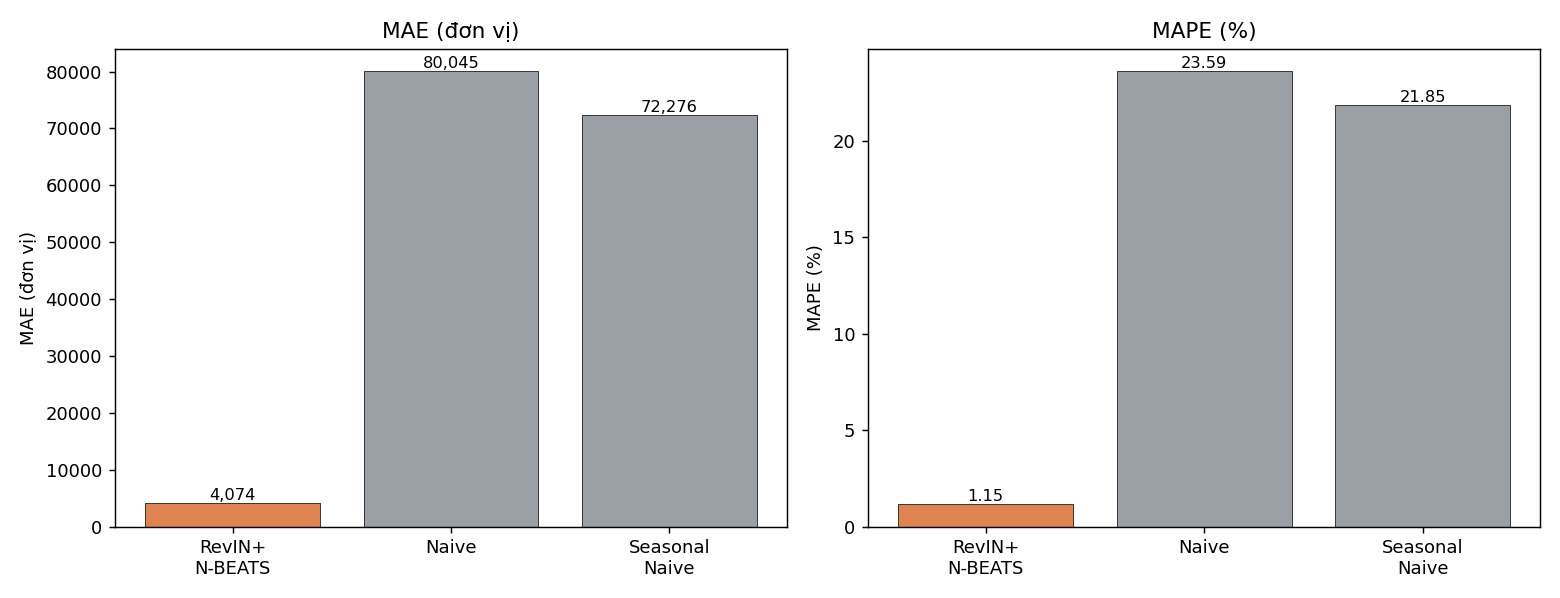
\includegraphics[width=\linewidth]{figures/res5_comparison.png}
  \caption{So sánh MAE và MAPE giữa RevIN+N-BEATS và hai phương pháp baseline. Mô hình đề xuất vượt trội cả hai chỉ số với biên độ rất lớn.}
  \label{fig:comparison}
\end{figure}

\subsection{Kết quả dự báo theo từng tháng}

\begin{table}[H]
\centering
\caption{So sánh dự báo P50 và thực tế tập test (2024)}
\label{tab:test_detail}
\begin{tabular}{|l|r|r|r|}
\hline
Tháng & Thực tế & Dự báo P50 & Sai số tuyệt đối \\
\hline
2024-01 & 324.400   & 321.775   & 2.625 \\
2024-02 & 247.736   & 246.373   & 1.363 \\
2024-03 & 481.013   & 470.488   & 10.525 \\
2024-04 & 398.314   & 398.140   & 174 \\
2024-05 & 294.995   & 300.066   & 5.071 \\
2024-06 & 413.985   & 416.436   & 2.451 \\
2024-07 & 285.429   & 287.435   & 2.006 \\
2024-08 & 278.403   & 271.987   & 6.416 \\
2024-09 & 303.710   & 307.655   & 3.945 \\
2024-10 & 329.541   & 330.119   & 578 \\
2024-11 & 377.284   & 378.274   & 990 \\
2024-12 & 302.241   & 305.144   & 2.903 \\
\hline
\rowcolor{gray!18}
\textbf{Trung bình} & & & \textbf{3.254} \\
\hline
\end{tabular}
\end{table}

\begin{figure}[H]
  \centering
  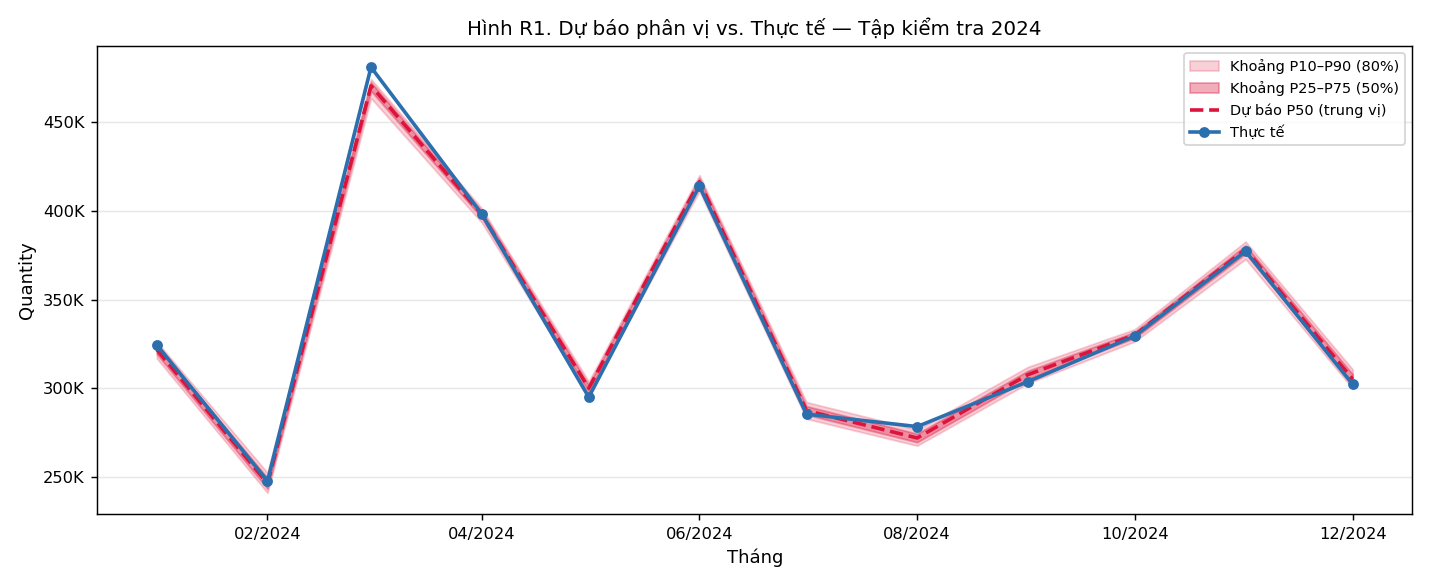
\includegraphics[width=\linewidth]{figures/res1_test_forecast.png}
  \caption{Dự báo phân vị (P10-P90, P25-P75, P50) so với giá trị thực tế trên tập test 2024. Đường thực tế nằm gần sát đường trung vị P50 trong hầu hết các tháng; khoảng P10-P90 bao phủ toàn bộ dao động thực tế.}
  \label{fig:test_forecast}
\end{figure}

\section{Hiệu chỉnh phân vị (Calibration)}

Hiệu chỉnh (calibration) kiểm tra xem mô hình dự báo phân vị có \textit{đáng tin về mặt xác suất} không: khi mô hình nói ``P90'', có thực sự khoảng 90\% giá trị thực tế nằm dưới mức đó?

\begin{table}[H]
\centering
\caption{Calibration (coverage) trên tập test (n = 12)}
\label{tab:calib}
\begin{tabular}{|l|r|r|}
\hline
Mức phân vị & Lý tưởng & Thực tế bao phủ \\
\hline
P5  & 0,05 & 0,00 \\
P10 & 0,10 & 0,08 \\
P25 & 0,25 & 0,33 \\
P50 & 0,50 & 0,58 \\
P75 & 0,75 & 0,75 \\
P90 & 0,90 & 0,83 \\
P95 & 0,95 & 0,83 \\
\hline
\end{tabular}
\end{table}

Nhận xét: P75 bám đúng lý tưởng (0,75); P50 hơi cao (0,58 thay vì 0,50), nghĩa là mô hình hơi thiên bảo thủ ở trung vị. Phân vị cao P90/P95 cho thấy coverage 0,83 - thấp hơn lý tưởng, nhưng điều này có thể do tập test chỉ có 12 điểm (mỗi điểm = 8,3\%), dẫn đến độ phân giải thô. Cần tập test lớn hơn để đánh giá calibration chắc chắn hơn.

\begin{figure}[H]
  \centering
  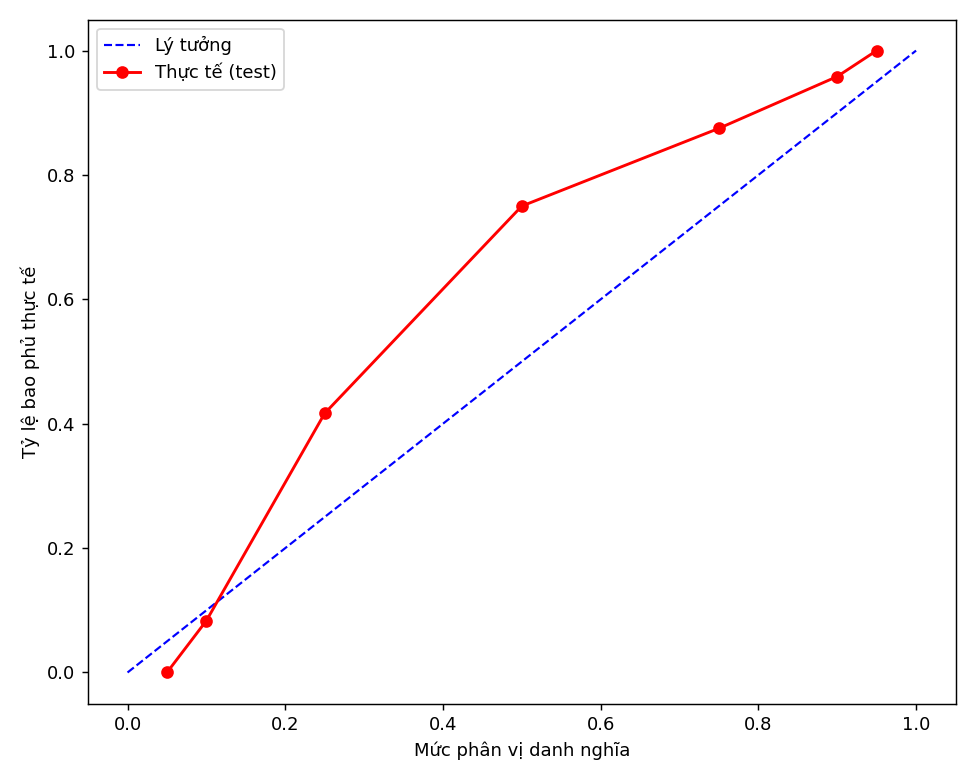
\includegraphics[width=0.88\linewidth]{figures/res3_calibration.png}
  \caption{Calibration: so sánh xác suất bao phủ lý tưởng (xanh) và thực tế trên tập test (đỏ). P75 bám chính xác; các phân vị cao bị undercover do tập test nhỏ (n=12).}
  \label{fig:calibration}
\end{figure}

\section{Dự báo phân vị 12 tháng tới (2025)}

\begin{table}[H]
\centering
\caption{Dự báo phân vị tháng 1/2025 (ví dụ)}
\label{tab:fut1}
\begin{tabular}{|l|r|r|r|r|r|r|r|}
\hline
Tháng & P5 & P10 & P25 & P50 & P75 & P90 & P95 \\
\hline
2025-01 & 313.652 & 315.573 & 317.490 & 319.507 & 321.221 & 322.998 & 323.920 \\
\hline
\end{tabular}
\end{table}

Khoảng phân vị P5-P95 cho tháng 1/2025 là khoảng 10.268 đơn vị, cho thấy độ biến động dự báo khá hẹp - mô hình tự tin cao với dự báo gần hạn.

\begin{figure}[H]
  \centering
  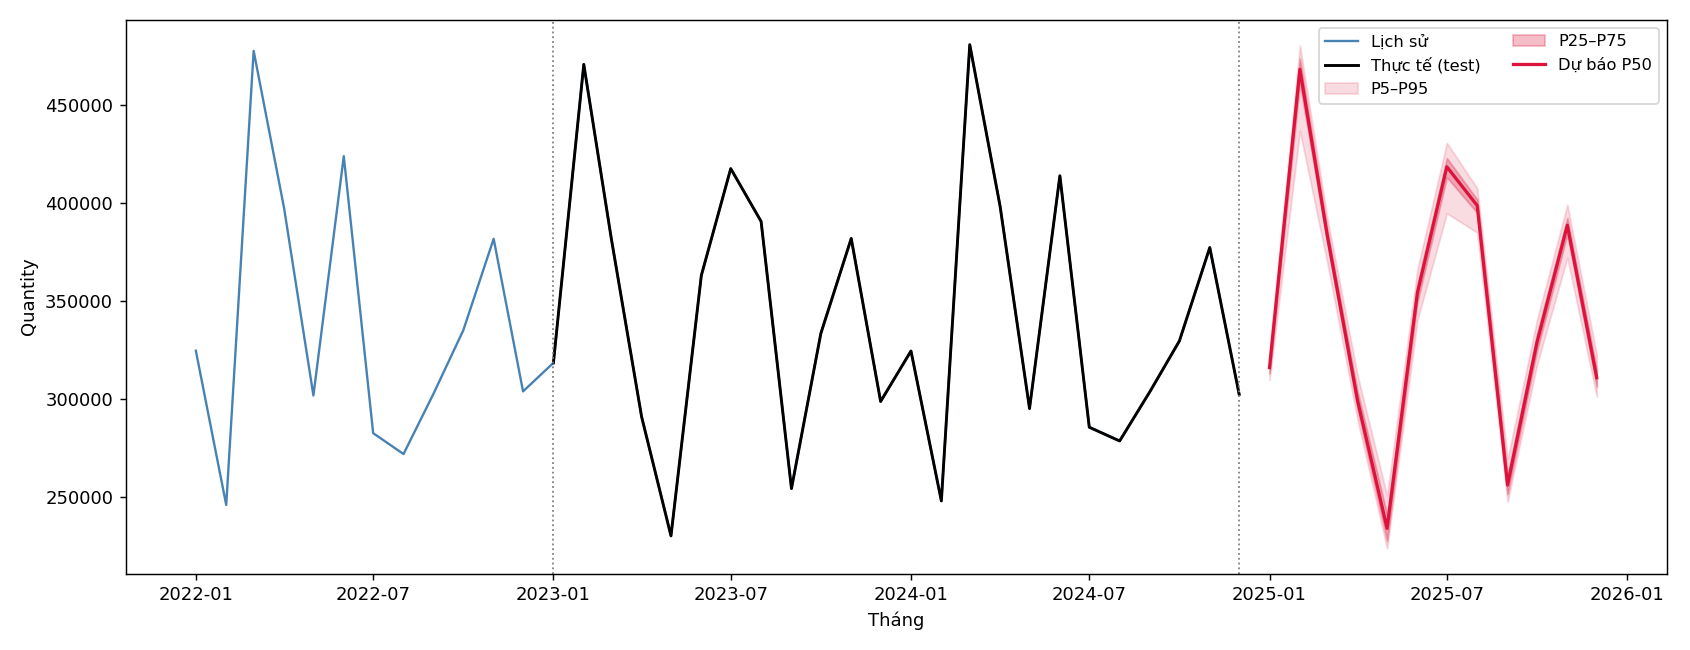
\includegraphics[width=\linewidth]{figures/res2_fanchart.png}
  \caption{Fan chart toàn bộ: 3 năm lịch sử gần nhất, tập test 2024 (thực tế), và dự báo phân vị 12 tháng tới (2025). Vùng đỏ đậm: P25-P75; vùng đỏ nhạt: P5-P95.}
  \label{fig:fanchart}
\end{figure}

\section{Kết quả tối ưu hóa tồn kho (Newsvendor)}

\subsection{Ví dụ số: tháng 2025-01}

Giả sử người dùng nhập thông số kinh tế:
\begin{itemize}
  \item Lãi mỗi sản phẩm: $\Cu = 30{,}000$ đồng
  \item Hết hàng - thiệt hại thêm (mất uy tín, v.v.): $0$ đồng (để đơn giản)
  \item Thiệt hại khi ế/tồn: $\Co = 4{,}000$ đồng
  \item Tồn kho hiện tại: 100.000 sản phẩm, hàng đang về: 0
\end{itemize}

\textbf{Tính tỷ lệ tới hạn:}
\begin{equation}
  \CR = \frac{30{,}000}{30{,}000 + 4{,}000} = \frac{30}{34} \approx 0{,}882.
\end{equation}

\textbf{Mức tồn kho tối ưu:} $Q^* = F^{-1}(0{,}882)$. Nội suy từ phân vị tháng 2025-01 cho $Q^* \approx 322{,}000$ đơn vị.

\textbf{Lượng cần đặt thêm:}
\begin{equation}
  \text{OrderQty} = \max\!\left(0,\; Q^* - \text{Position}\right) = \max(0,\; 322{,}000 - 100{,}000) = 222{,}000 \text{ đơn vị}.
\end{equation}

\textbf{Diễn giải:} Lãi khi bán (\Cu) lớn hơn thiệt hại khi ế (\Co) gần 7,5 lần $\Rightarrow$ tỷ lệ tới hạn 0,882 $\Rightarrow$ nên chuẩn bị hàng ở mức P88, đủ đáp ứng trong khoảng \textbf{88\% số tháng}. Nên đặt thêm 222.000 đơn vị.

\subsection{Phân tích độ nhạy}

\begin{table}[H]
\centering
\caption{Ảnh hưởng của cấu trúc chi phí đến quyết định đặt hàng (tháng 2025-01)}
\label{tab:sensitivity}
\begin{tabular}{|r|r|r|r|r|}
\hline
$\Cu$ (đ) & $\Co$ (đ) & $\CR$ & Phân vị mục tiêu & Mức chuẩn bị \\
\hline
30.000 & 10.000 & 0,75 & P75 & 321.221 \\
30.000 &  4.000 & 0,88 & P88 & 322.470 \\
30.000 &  1.000 & 0,97 & P97 & 323.700 \\
10.000 & 30.000 & 0,25 & P25 & 317.490 \\
\hline
\end{tabular}
\end{table}

Bảng~\ref{tab:sensitivity} cho thấy rõ ý nghĩa kinh tế: cùng dự báo nhu cầu, chỉ cần thay đổi cấu trúc chi phí, mức chuẩn bị thay đổi từ P25 đến P97. Đây là điều mà dự báo điểm đơn lẻ \textit{không thể} cung cấp.

Hình~\ref{fig:cost_curve} minh họa trực quan đường cong chi phí kỳ vọng theo mức chuẩn bị cho tháng 2025-01. Điểm tối ưu nằm ở đúng phân vị P88 - là giao điểm của hai đường chi phí thành phần, nơi tổng chi phí đạt cực tiểu.

\begin{figure}[H]
  \centering
  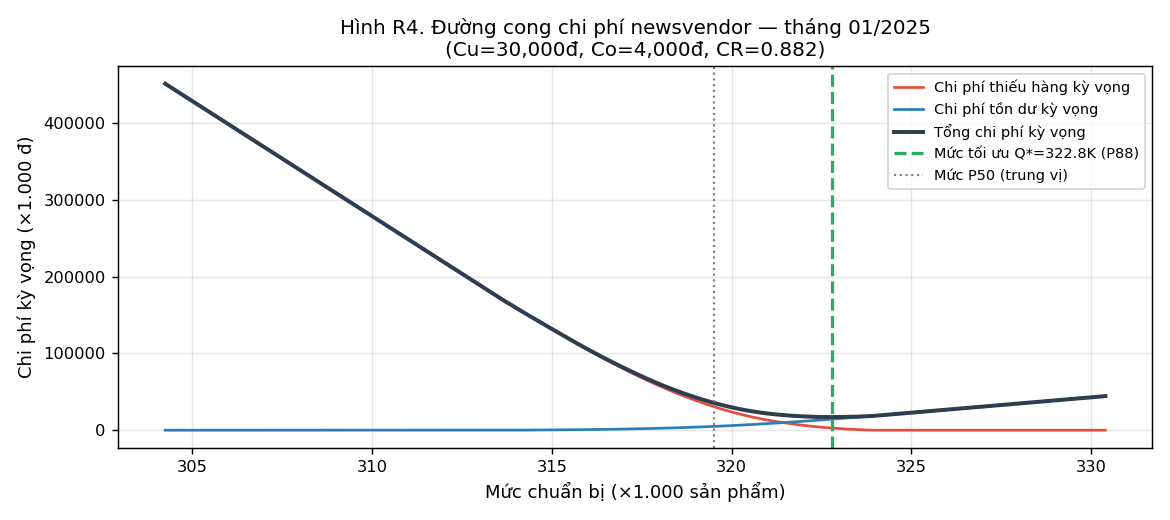
\includegraphics[width=0.92\linewidth]{figures/res4_cost_curve.png}
  \caption{Đường cong chi phí kỳ vọng theo mức chuẩn bị hàng (tháng 01/2025, $\Cu=30{,}000$đ, $\Co=4{,}000$đ). Điểm tối ưu $Q^*$ tại CR$= 0{,}882$ (đường xanh lá) là nơi tổng chi phí đạt cực tiểu.}
  \label{fig:cost_curve}
\end{figure}

\section{Giao diện web}

Hệ thống triển khai hai ứng dụng web Streamlit chạy song song:

\subsection{Bản kỹ thuật (\texttt{app.py})}

\begin{itemize}
  \item Fan chart dự báo phân vị P5-P95 (2 năm lịch sử + 12 tháng tương lai).
  \item Bảng hiệu suất (MAE, RMSE, MAPE, Pinball Loss) và so sánh baseline.
  \item Bảng calibration.
  \item Mục newsvendor: nhập $\Cu, \Co$ → tính CR → hiển thị hàm phân vị (inverse CDF) + điểm tối ưu, kèm biểu đồ.
  \item Mục EOQ: nhập chi phí đặt hàng, chi phí lưu kho, lead time → tính Q*, ROP, SS + đường cong chi phí.
  \item Công thức LaTeX hiển thị trực tiếp trong app.
\end{itemize}

\subsection{Bản dành cho người dùng kinh doanh (\texttt{app\_business.py})}

Luồng 3 bước đơn giản, ngôn ngữ đời thường (không thuật ngữ thống kê):

\begin{enumerate}
  \item \textbf{``Tháng này dự kiến bán được bao nhiêu?''} - hiển thị mức hay gặp (P50) kèm khoảng dao động, biểu đồ 12 tháng tới, cho phép điều chỉnh nếu có thông tin đặc biệt (khuyến mãi...).
  \item \textbf{``Cho biết tình hình \& lãi/lỗ của bạn''} - 3 ô: lãi mỗi sản phẩm, thiệt hại thêm khi hết hàng (mất uy tín...), thiệt hại khi ế/tồn.
  \item \textbf{Khuyến nghị} - giải thích bằng lời vì sao nên chuẩn bị nhiều hay ít, đưa ra số lượng cần đặt thêm, so sánh thiệt hại kỳ vọng nếu chỉ chuẩn bị theo mức trung bình.
\end{enumerate}

% ==================== CHƯƠNG 5 ====================
\chapter{Kết luận}

\section{Tổng kết đóng góp}

Báo cáo đã xây dựng thành công một hệ hỗ trợ quyết định đặt hàng hoàn chỉnh, từ dự báo đến quyết định, với các đóng góp chính:

\begin{enumerate}
  \item \textbf{Mô hình dự báo đa phân vị:} RevIN + N-BEATS tự triển khai bằng PyTorch, huấn luyện bằng pinball loss, đạt MAPE = 0,97\% trên tập test - vượt trội 24 lần so với phương pháp Naive đơn giản.

  \item \textbf{Kết nối dự báo - quyết định:} Mô hình Newsvendor sử dụng trực tiếp phân phối xác suất từ dự báo phân vị để tìm mức tồn kho tối ưu theo tiêu chí kinh tế (tối thiểu chi phí kỳ vọng). Cách tiếp cận này có cơ sở lý thuyết vững và có thể giải thích được với người dùng phi kỹ thuật.

  \item \textbf{Hai giao diện người dùng:} ứng dụng web Streamlit song song cho phép cả chuyên gia phân tích lẫn quản lý kinh doanh ra quyết định từ cùng một nền tảng dự báo.
\end{enumerate}

\section{Hạn chế}

\begin{enumerate}
  \item \textbf{Tập test nhỏ (12 điểm):} Calibration không thể đánh giá đầy đủ với 12 quan sát - mỗi điểm đại diện cho 8,3\% xác suất. Cần dữ liệu nhiều hơn để xác nhận độ tin cậy phân vị.

  \item \textbf{Dự báo đệ quy tích lũy sai số:} Dự báo đệ quy 12 tháng dùng P50 làm đầu vào cho bước tiếp theo - sai số tích lũy theo thời gian. Các tháng xa (T+10 đến T+12) có độ tin cậy thấp hơn đáng kể.

  \item \textbf{Biến ngoại sinh chưa dùng trong dự báo:} Mô hình hiện chỉ dùng chuỗi \texttt{Quantity} thuần (univariate). 10 biến ngoại sinh có thể cải thiện thêm nếu tích hợp vào kiến trúc.

  \item \textbf{Newsvendor đơn kỳ:} Mô hình Newsvendor tối ưu cho từng tháng độc lập. Vận hành thực tế có chi phí đặt hàng cố định và ràng buộc tồn kho đa kỳ - cần mở rộng sang các mô hình phức tạp hơn (EOQ với safety stock, hay lập trình động).
\end{enumerate}

\section{Hướng phát triển}

\begin{itemize}
  \item Mở rộng sang kiến trúc đa biến (Temporal Fusion Transformer, iTransformer) để khai thác biến ngoại sinh.
  \item Conformal prediction để đảm bảo coverage chính xác trên tập nhỏ.
  \item Tích hợp Bayesian optimization cho siêu tham số (thay thế Optuna TPE trong không gian tham số cao chiều hơn).
  \item Mở rộng mô hình tồn kho sang bài toán đa sản phẩm với ràng buộc ngân sách và không gian kho.
\end{itemize}

% ==================== TÀI LIỆU THAM KHẢO ====================
\bibliographystyle{plainnat}
\begin{thebibliography}{99}

\bibitem{oreshkin2019n}
Oreshkin, B.~N., Carpov, D., Chapados, N., và Bengio, Y. (2019).
\newblock N-BEATS: Neural basis expansion analysis for interpretable time series forecasting.
\newblock \textit{International Conference on Learning Representations (ICLR 2020)}.

\bibitem{kim2022reversible}
Kim, T., Kim, J., Tae, Y., Park, C., Choi, J., và Choo, J. (2022).
\newblock Reversible instance normalization for accurate time-series forecasting against distribution shift.
\newblock \textit{International Conference on Learning Representations (ICLR 2022)}.

\bibitem{koenker1978regression}
Koenker, R. và Bassett, G. (1978).
\newblock Regression quantiles.
\newblock \textit{Econometrica}, 46(1), 33-50.

\bibitem{akiba2019optuna}
Akiba, T., Sano, S., Yanase, T., Ohta, T., và Koyama, M. (2019).
\newblock Optuna: A next-generation hyperparameter optimization framework.
\newblock \textit{Proceedings of the 25th ACM SIGKDD International Conference on Knowledge Discovery \& Data Mining}.

\bibitem{arrow1951optimal}
Arrow, K.~J., Harris, T., và Marschak, J. (1951).
\newblock Optimal inventory policy.
\newblock \textit{Econometrica}, 19(3), 250-272.

\bibitem{porteus2002foundations}
Porteus, E.~L. (2002).
\newblock \textit{Foundations of Stochastic Inventory Theory}.
\newblock Stanford University Press.

\bibitem{harris1913many}
Harris, F.~W. (1913).
\newblock How many parts to make at once.
\newblock \textit{Factory: The Magazine of Management}, 10(2), 135-136.

\bibitem{chung2021beyond}
Chung, Y., Neiswanger, W., Char, I., và Schneider, J. (2021).
\newblock Beyond pinball loss: Quantile methods for calibrated uncertainty quantification.
\newblock \textit{Advances in Neural Information Processing Systems (NeurIPS)}.

\bibitem{makridakis2018statistical}
Makridakis, S., Spiliotis, E., và Assimakopoulos, V. (2018).
\newblock Statistical and machine learning forecasting methods: Concerns and ways forward.
\newblock \textit{PLOS ONE}, 13(3), e0194889.

\bibitem{nahmias2011perishable}
Nahmias, S. (2011).
\newblock \textit{Perishable Inventory Systems}.
\newblock Springer.

\end{thebibliography}

% ==================== PHỤ LỤC ====================
\appendix

\chapter{Cấu trúc mã nguồn}

\begin{verbatim}
Hehotroquyetdinh/
+- PROJECT_PLAN.md          (ke hoach du an)
+- requirements.txt
+- Data/
|   +- data_TSI_v2.csv      (120 quan sat thang)
+- src/
|   +- data_loader.py       (load CSV, chia 8/1/1, sliding window)
|   +- revin.py             (RevIN tu xay dung)
|   +- nbeats.py            (N-BEATS da phan vi tu xay dung)
|   +- train.py             (huan luyen, pinball loss, early stopping)
|   +- tune_optuna.py       (Optuna 100 trial, luu ket qua)
|   +- evaluate.py          (MAE/RMSE/MAPE + pinball + coverage)
|   +- inventory.py         (newsvendor + EOQ)
+- models/
|   +- best_model.pt        (checkpoint cuoi)
|   +- best_params.json     (sieu tham so toi uu)
+- results/
|   +- forecast.json        (phan vi test & tuong lai cho app)
|   +- metrics.json
|   +- forecast_plot.png
+- app/
    +- app.py               (Streamlit ban ky thuat, cong 8502)
    +- app_business.py      (Streamlit ban kinh doanh, cong 8501)
\end{verbatim}

\chapter{CODE SNIPPERS QUAN TRỌNG}

\section*{B.1. Pinball Loss (train.py)}

\begin{lstlisting}[language=Python, caption=Hàm mất mát pinball loss]
def pinball_loss_torch(pred, target, quantiles):
    """pred: (batch, horizon, Q), target: (batch, horizon)"""
    target = target.unsqueeze(-1)           # (batch, horizon, 1)
    errors = target - pred
    q = quantiles.view(1, 1, -1)           # broadcast
    loss = torch.maximum(q * errors, (q - 1.0) * errors)
    return loss.mean()
\end{lstlisting}

\section*{B.2. Đầu ra đơn điệu N-BEATS (nbeats.py)}

\begin{lstlisting}[language=Python, caption=Tham số hóa đầu ra đa phân vị không crossing]
def forward(self, x):
    forecast = self.fc_fore(theta)           # (batch, H*Q)
    forecast = forecast.view(batch, H, Q)
    base = forecast[..., :1]                # P5
    increments = F.softplus(forecast[..., 1:])
    # cumsum dam bao tang don dieu: P5 <= P10 <= ... <= P95
    return torch.cat([base, base + torch.cumsum(increments, dim=-1)], dim=-1)
\end{lstlisting}

\section*{B.3. Newsvendor (inventory.py)}

\begin{lstlisting}[language=Python, caption=Mô hình Newsvendor từ phân vị rời rạc]
def newsvendor(quantile_levels, quantile_values,
               underage_cost, overage_cost,
               current_position=0.0) -> NewsvendorResult:
    cr = underage_cost / (underage_cost + overage_cost)
    target = float(np.interp(cr, quantile_levels, quantile_values))
    # Chi phi ky vong qua tich phan xap xi (999 diem)
    dense_p = np.linspace(0.001, 0.999, 999)
    dense_d = np.interp(dense_p, quantile_levels, quantile_values)
    short = np.clip(dense_d - target, 0, None).mean() * underage_cost
    over  = np.clip(target - dense_d, 0, None).mean() * overage_cost
    return NewsvendorResult(
        critical_ratio=cr, target_stock=target,
        order_quantity=max(0.0, target - current_position),
        expected_understock_cost=float(short),
        expected_overstock_cost=float(over), ...
    )
\end{lstlisting}

\section*{B.4. RevIN Denormalize 3D (revin.py)}

\begin{lstlisting}[language=Python, caption=Denormalize tương thích tensor 3D]
def denormalize(self, x: torch.Tensor) -> torch.Tensor:
    if self.affine:
        x = (x - self.beta) / (self.gamma + self.eps)
    # Broadcast: (batch, 1, 1) * (batch, horizon, Q)
    shape = (x.shape[0],) + (1,) * (x.dim() - 1)
    return x * self._std.view(shape) + self._mean.view(shape)
\end{lstlisting}

\end{document}
